\section{Ensaios de Bancada com o Motor}
\label{sec:ensaios_bancada}

\subsection{Instrumentação dos Ensaios com o Motor em Rotação}
\label{sec:resultado_setup_scope}

Os ensaios com o motor girando foram conduzidos com um osciloscópio
PicoScope da Série 5000, disponível no laboratório do PET, operado pelo
programa de aquisição do próprio fabricante
(\autoref{fig:setup_picoscope_sw}). O equipamento oferece quatro canais
analógicos e dois canais digitais, e essa disponibilidade definiu a
divisão das grandezas registradas: duas tensões de fase e duas correntes
de fase nos canais analógicos; o comando enviado ao gerador de pulsos e o
sinal do tacômetro óptico nos canais digitais. As correntes vêm dos
sensores de efeito Hall da própria placa de medição, cuja saída em tensão
é lida diretamente pelo osciloscópio. A terceira tensão e a terceira
corrente não são medidas: com o enrolamento equilibrado e sem caminho de
retorno pelo neutro, ambas são reconstruídas na análise a partir das duas
registradas, já que as três somam zero a cada instante.


\begin{figure}[H]
    \centering
    \caption{Tela do PicoScope}
    \label{fig:setup_picoscope_sw}
    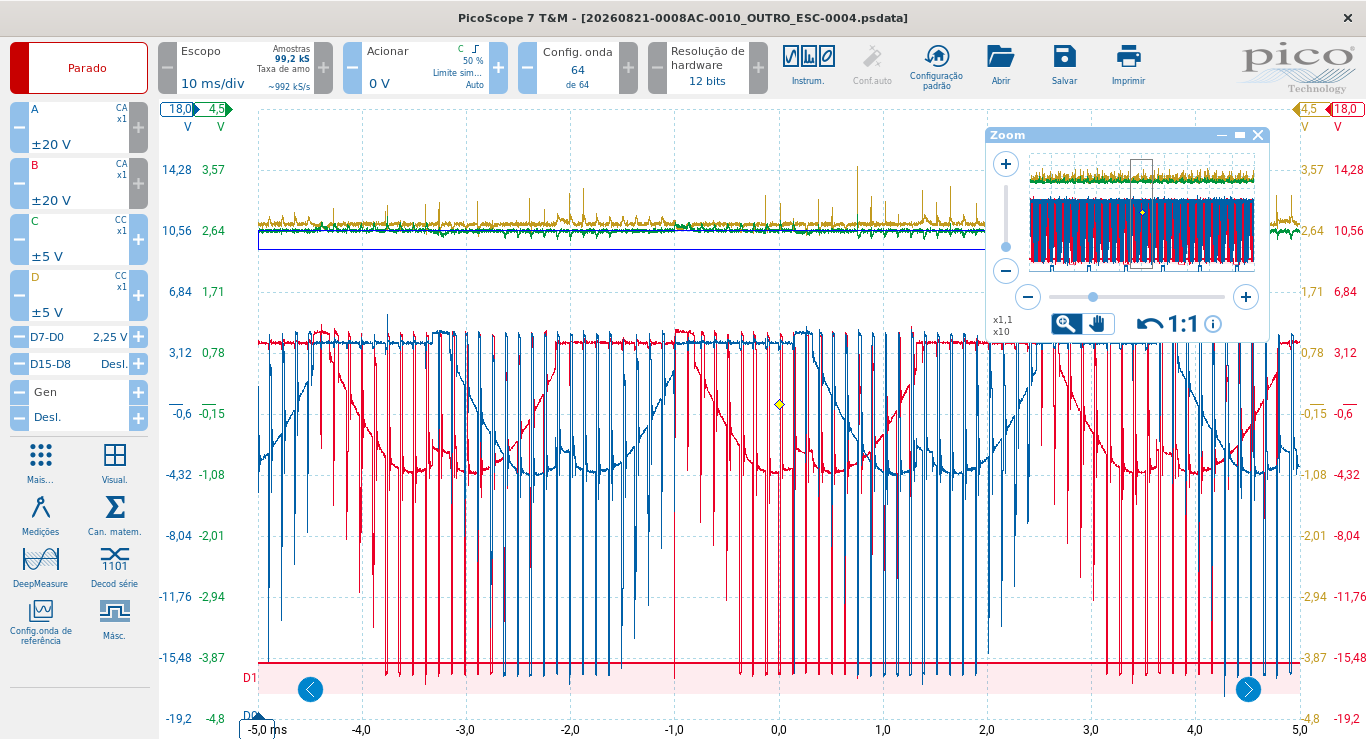
\includegraphics[width=0.9\linewidth]{Textuais/Imgs/Resultados/picoscope_software.png}

    Fonte: Autor (2026)
\end{figure}

A alimentação do conjunto foi feita por bateria, e não pela fonte de
rede. Com isso o barramento fica flutuante em relação ao terra da
instalação, o que evita laço de terra entre a alimentação do motor e a
referência das pontas de prova do osciloscópio, e elimina a ondulação
residual da retificação, que apareceria somada às tensões de fase
medidas. O acionamento coube a dois controladores eletrônicos de
velocidade distintos, empregados em sessões diferentes de ensaio: um Castle
Talon de \SI{90}{\ampere} e um Flycolor de \SI{150}{\ampere}.

O motor tem os enrolamentos ligados em estrela e não traz o ponto neutro
acessível externamente: só os três terminais de fase saem da carcaça.
Como as tensões de fase precisam ser medidas em relação ao neutro, ele foi
reconstruído por fora com três resistores de mesmo valor, um por fase,
unidos em um nó comum. Sendo iguais as resistências e equilibrado o
sistema, esse nó reproduz o potencial do neutro do enrolamento e serve de
referência para as pontas de prova, técnica corrente na medição de
máquinas em estrela com neutro inacessível \cite{nidec_neutral_point}. O
valor dos resistores é alto frente à impedância de fase, de modo que a
corrente desviada pelo divisor é desprezível diante da corrente do motor.
A \autoref{fig:setup_picoscope_fisico} mostra a montagem física do ensaio.


\begin{figure}[H]
    \centering
    \caption{Montagem física do ensaio: motor, bateria, neutro virtual e osciloscópio}
    \label{fig:setup_picoscope_fisico}
    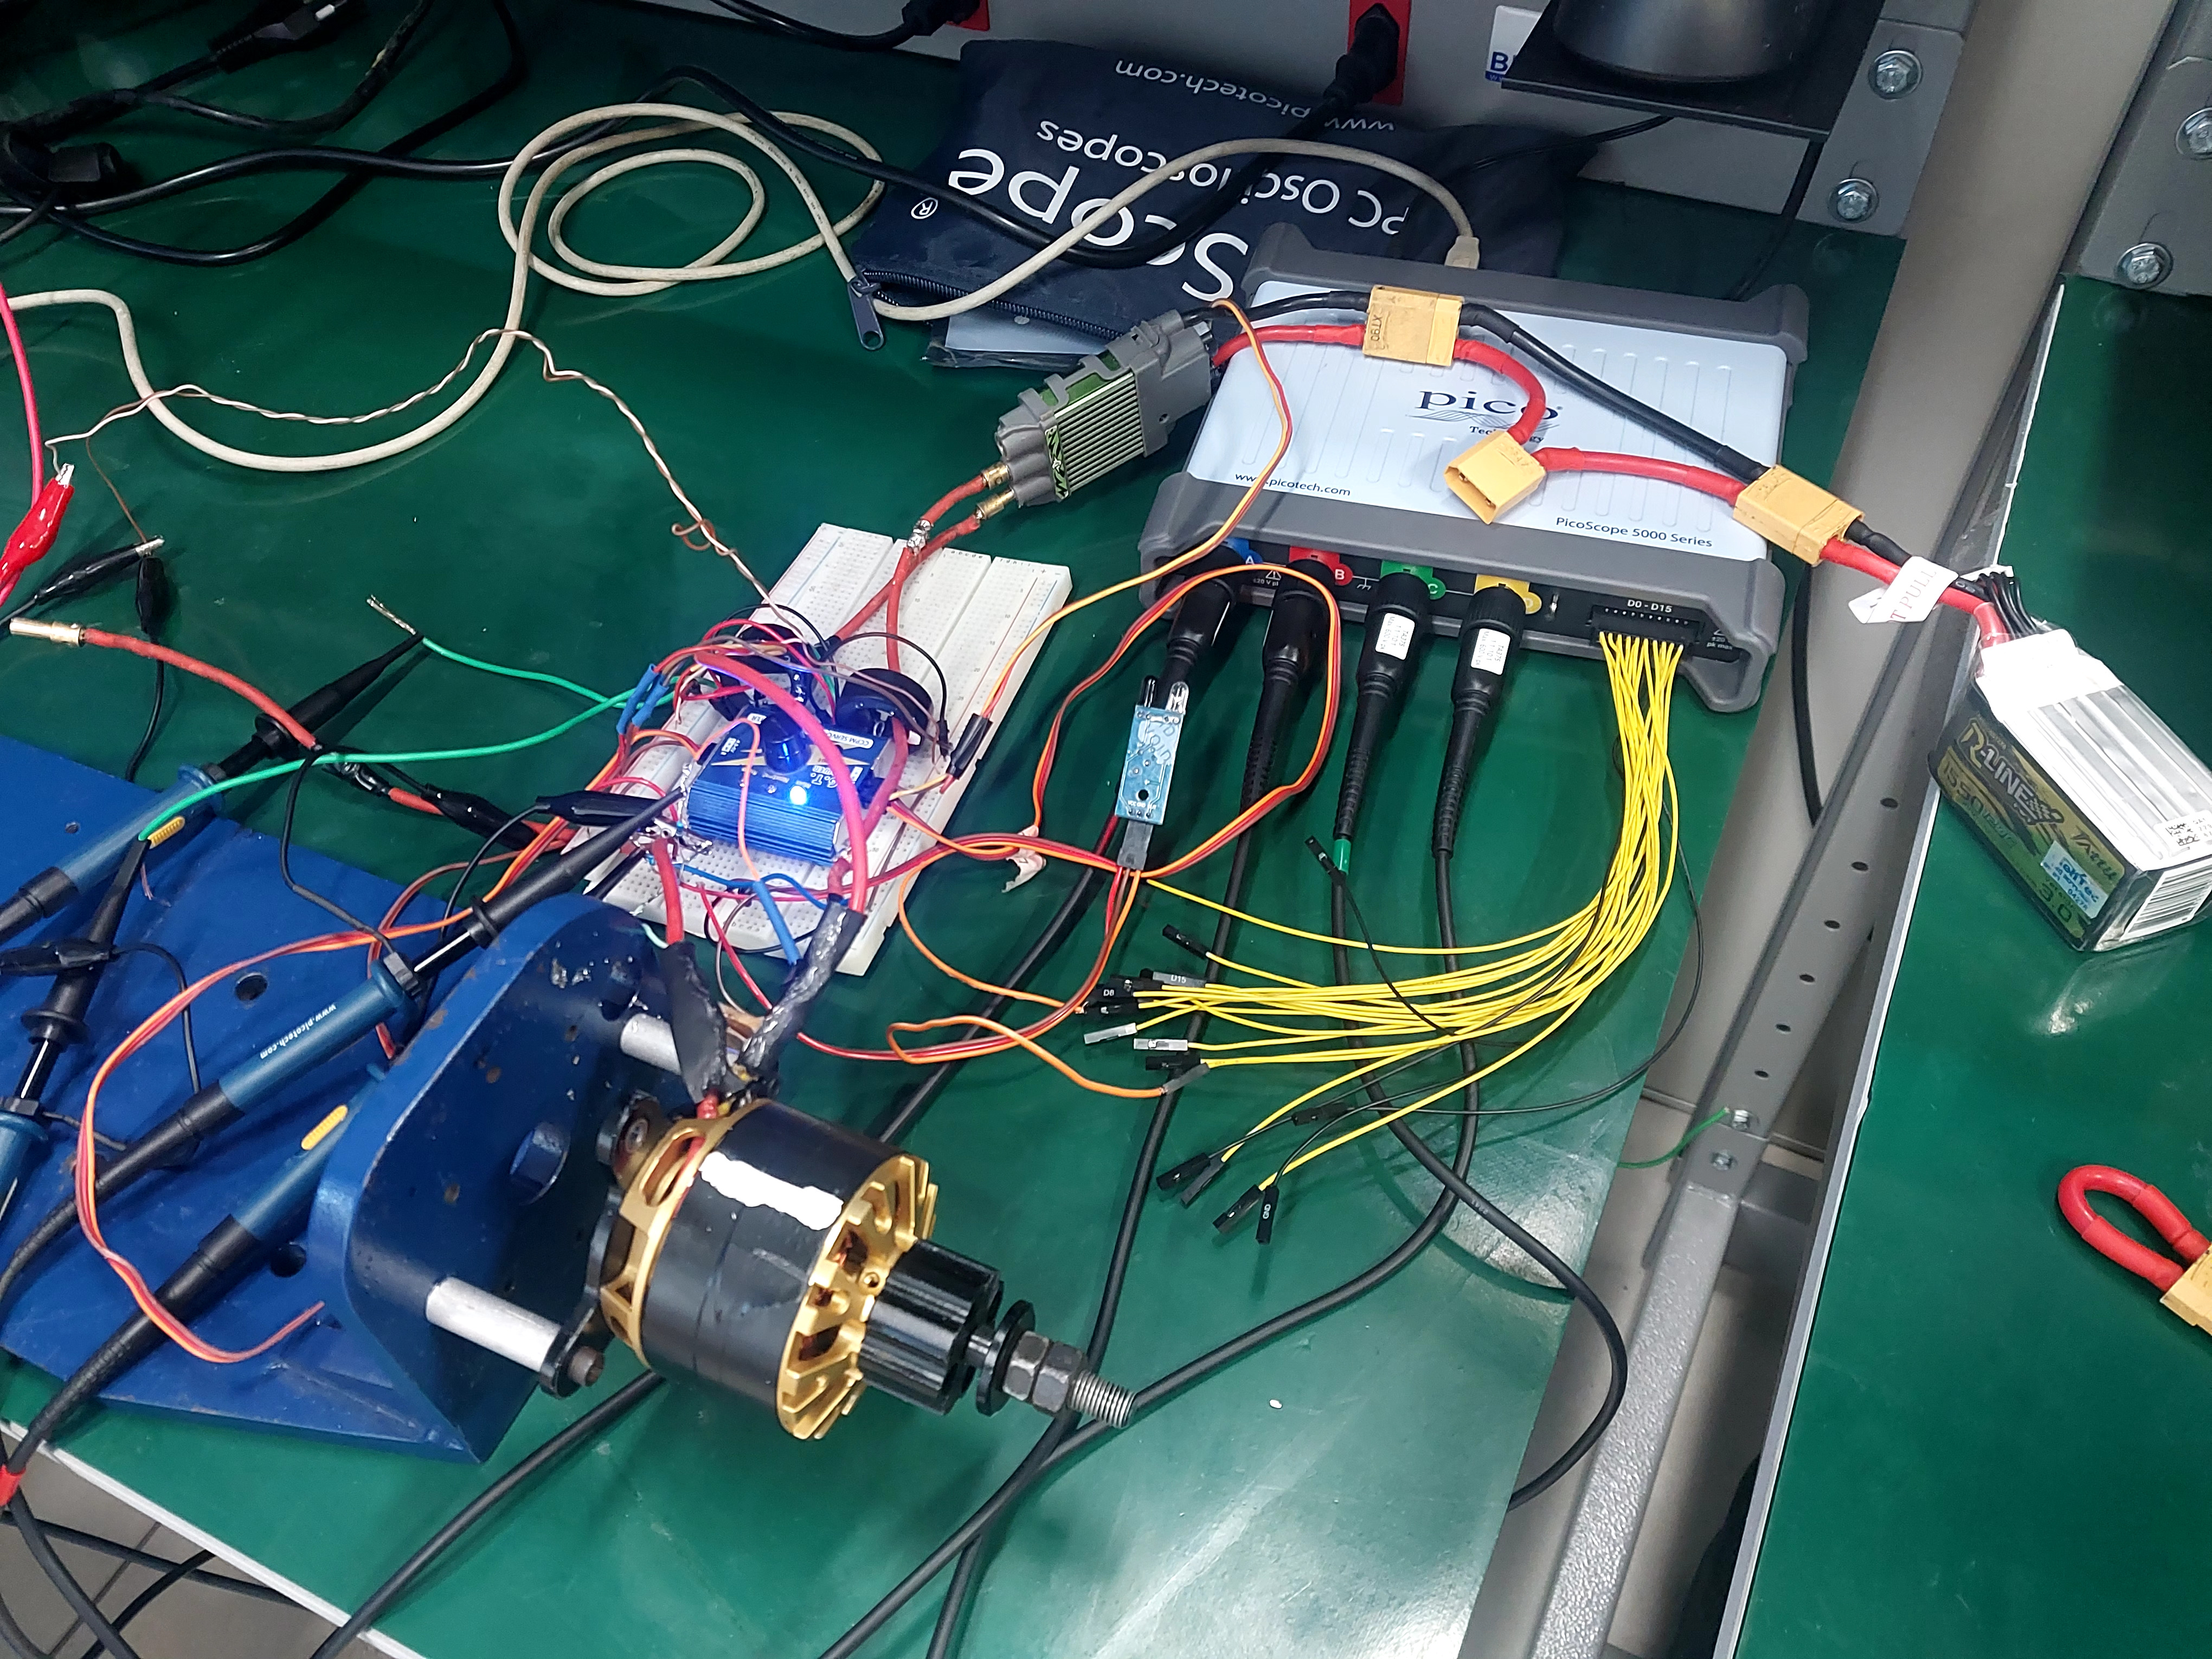
\includegraphics[width=0.85\linewidth]{Textuais/Imgs/Resultados/ensaio_motor_vazio.jpg}

    Fonte: Autor (2026)
\end{figure}

\subsection{Coeficientes Mecânicos}
\label{sec:resultado_coef_mec}

O levantamento das perdas mecânicas foi feito com o motor girando em vazio,
na montagem improvisada descrita na \autoref{sec:resultado_setup_scope}.
Foram registrados \num{19} patamares de rotação, de
\SI{130}{\radian\per\second} a \SI{705}{\radian\per\second}. Sem carga no
eixo, todo o torque desenvolvido é gasto nas perdas, de modo que o torque
medido em regime permanente é o próprio torque de perdas. Como a montagem
não dispõe de transdutor de torque, ele foi obtido pelo balanço de potência
por fase: a potência elétrica que entra no enrolamento, descontada a
dissipação resistiva, dividida pela velocidade mecânica. Esse caminho de
cálculo não exige conhecer a forma de onda da força contraeletromotriz, a
constante de FEM nem o ângulo do rotor, e é portanto independente do
observador avaliado na \autoref{sec:resultado_smo_bancada}. Os pontos
experimentais estão tabelados no \autoref{apendice:bancada}
(\autoref{tab:bancada_patamares}).

A \autoref{fig:bancada_te_omega} apresenta os pares
$(\omega_{m,k},\ T_{e,k})$ e a reta ajustada pela
Equação~\eqref{eq:ensaio_vazio_iq}. A regressão fornece

\begin{equation}
    B = (32{,}4 \pm 4{,}4)\times 10^{-6}~\si{\newton\meter\second\per\radian},
    \qquad
    \tau_c = (15{,}5 \pm 2{,}4)~\si{\milli\newton\meter},
    \label{eq:resultado_b_tauc}
\end{equation}

com coeficiente de determinação $R^2 = \num{0,925}$. As incertezas são os
erros padrão dos coeficientes da regressão.

\begin{figure}[H]
    \centering
    \caption{Torque de perdas em função da rotação e reta ajustada}
    \label{fig:bancada_te_omega}
    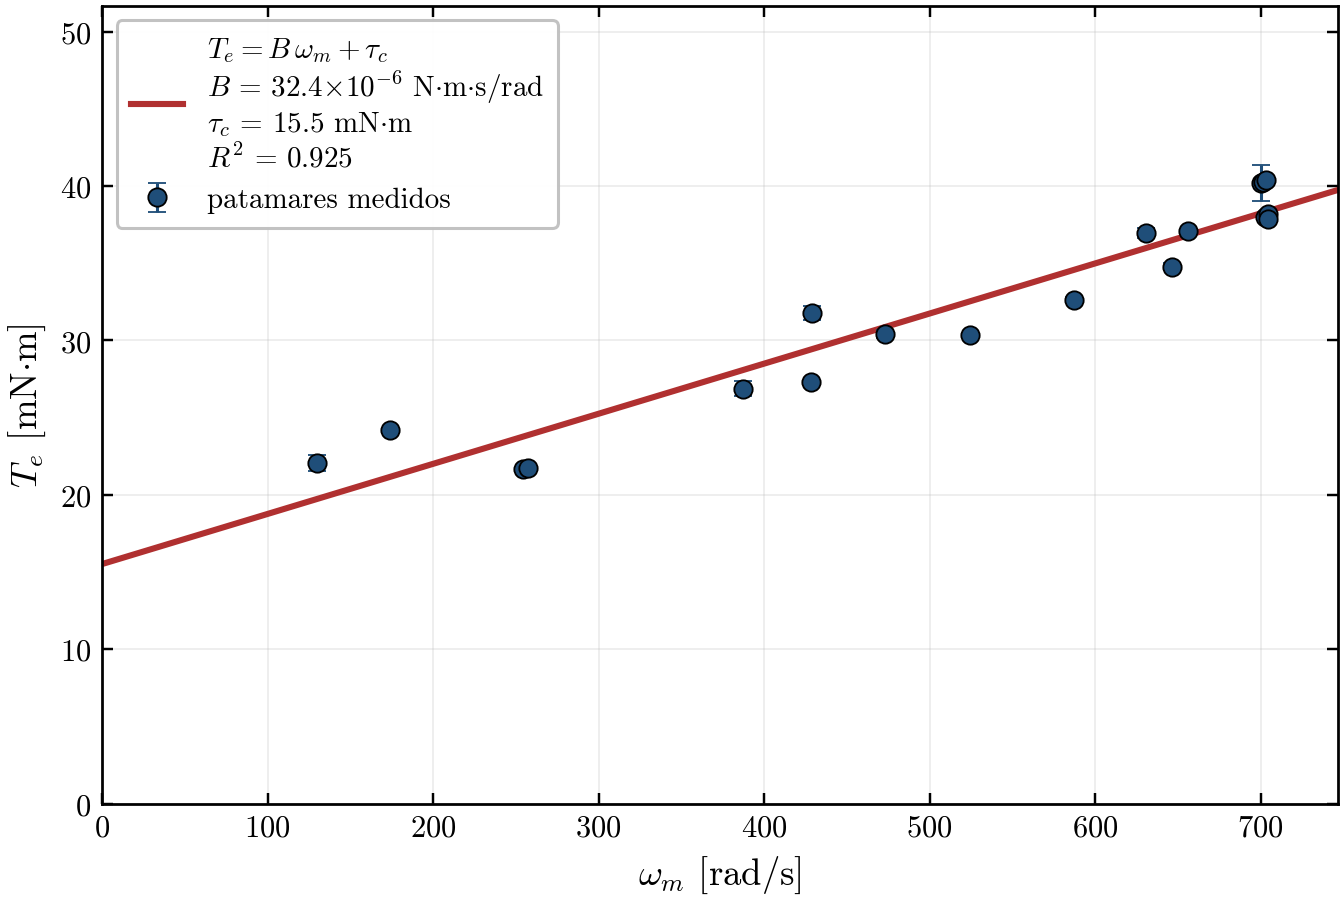
\includegraphics[width=0.9\linewidth]{Textuais/Imgs/Resultados/bancada_te_omega.png}

    Fonte: Autor (2026)
\end{figure}

Os resíduos da regressão (\autoref{fig:bancada_te_residuo}) distribuem-se em
torno de zero sem tendência aparente com a rotação, o que sugere que o
modelo de duas parcelas acompanha os dados na faixa ensaiada; o espalhamento
remanescente é da ordem da dispersão entre patamares.

\begin{figure}[H]
    \centering
    \caption{Resíduos da regressão do torque de perdas}
    \label{fig:bancada_te_residuo}
    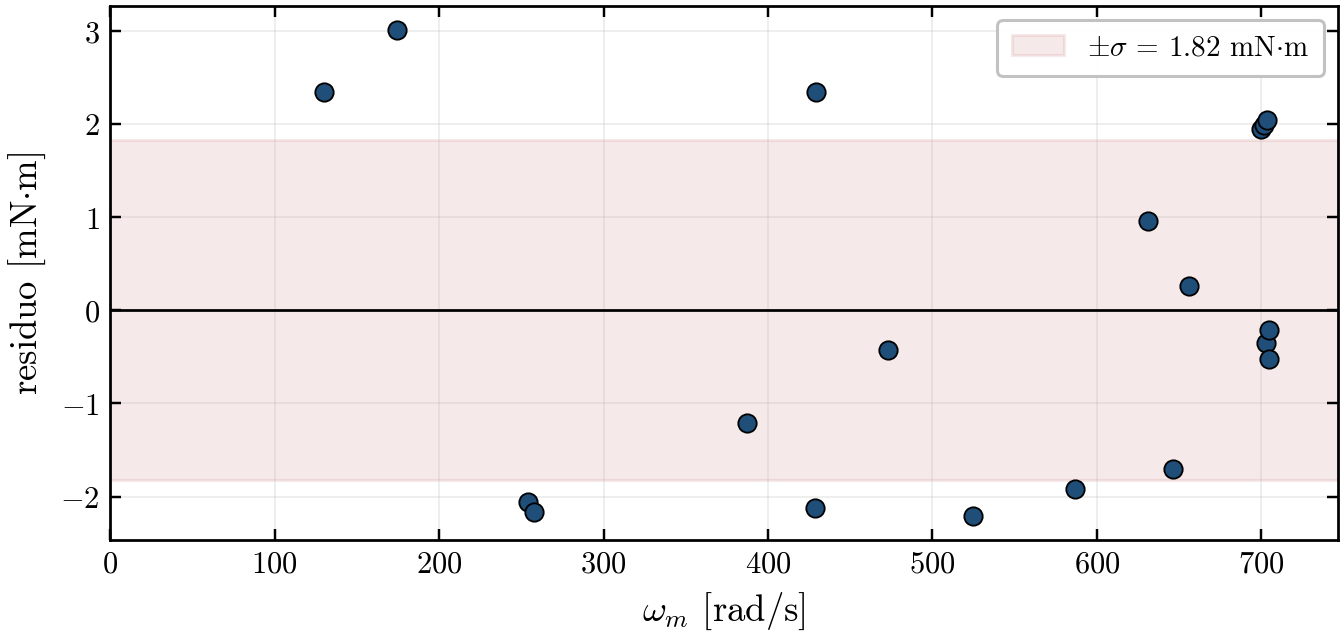
\includegraphics[width=0.9\linewidth]{Textuais/Imgs/Resultados/bancada_te_residuo.png}

    Fonte: Autor (2026)
\end{figure}

Chama a atenção o valor de $\tau_c$, alto para um motor deste porte se
interpretado apenas como atrito de Coulomb dos rolamentos. Uma explicação
plausível é a perda por histerese no ferro do estator: ela cresce
proporcionalmente à rotação e, portanto, aparece na regressão como um torque
constante, somando-se ao atrito seco. Sob essa leitura, os dois coeficientes
não seriam grandezas puramente mecânicas --- $\tau_c$ reuniria o atrito seco
dos rolamentos e a histerese, e $B$ reuniria o atrito viscoso, a ventilação e
a perda por corrente parasita. Para o uso pretendido, que é prever o torque de
perdas a ser descontado na estimação, o modelo agregado atende, pois o que
interessa é a soma das perdas independentes de carga.

A medida de rotação, da qual todo o levantamento depende, foi conferida
contra a frequência elétrica extraída das tensões de fase. Sobre \num{267}
registros, o desvio médio entre as duas leituras é
$-7{,}9\times10^{-4}\,\%$, com desvio padrão de $3{,}7\times10^{-2}\,\%$
(\autoref{fig:bancada_tacometro}). O resultado é compatível com um pulso por
volta no disco do tacômetro e sete pares de polos no rotor, pressupostos
usados na conversão entre velocidade elétrica e mecânica ao longo do
trabalho. Esse e os demais valores consolidados do ensaio estão
reunidos na \autoref{tab:bancada_parametros}, no \autoref{apendice:bancada}.

\begin{figure}[H]
    \centering
    \caption{Validação do tacômetro óptico contra a frequência elétrica das tensões de fase}
    \label{fig:bancada_tacometro}
    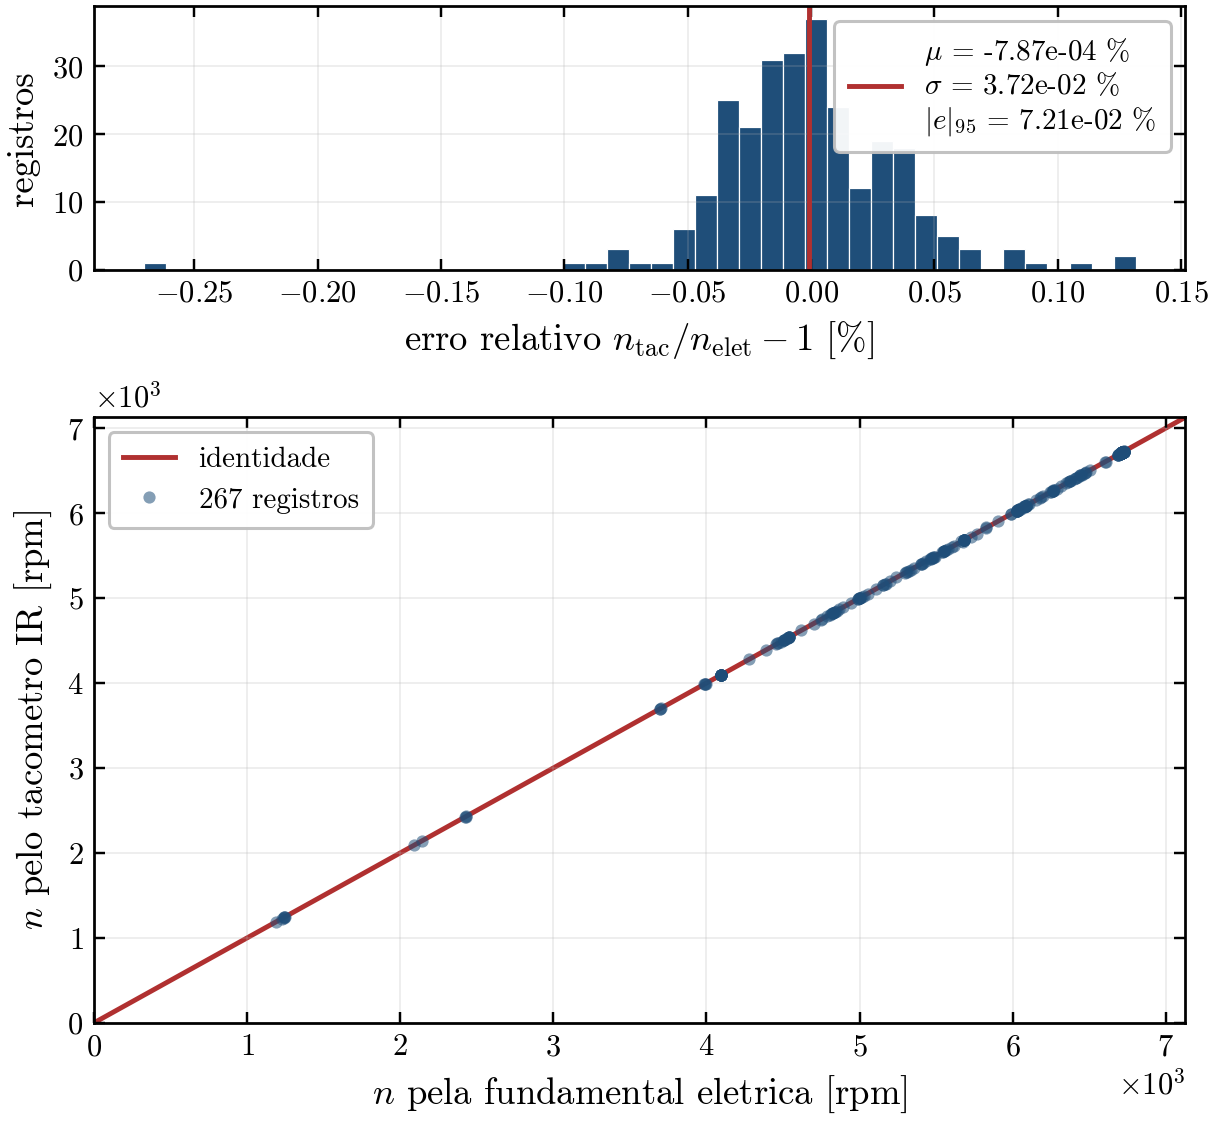
\includegraphics[width=0.9\linewidth]{Textuais/Imgs/Resultados/bancada_tacometro.png}

    Fonte: Autor (2026)
\end{figure}

A constante de força contraeletromotriz foi extraída dos mesmos registros,
pela razão entre a amplitude da FEM e a velocidade elétrica, patamar a
patamar (\autoref{fig:bancada_ke}). O valor obtido é estável ao longo da
faixa e equivale a \num{310}~RPM/V, valor próximo da especificação de placa
do motor.

\begin{figure}[H]
    \centering
    \caption{Constante de força contraeletromotriz em função da rotação}
    \label{fig:bancada_ke}
    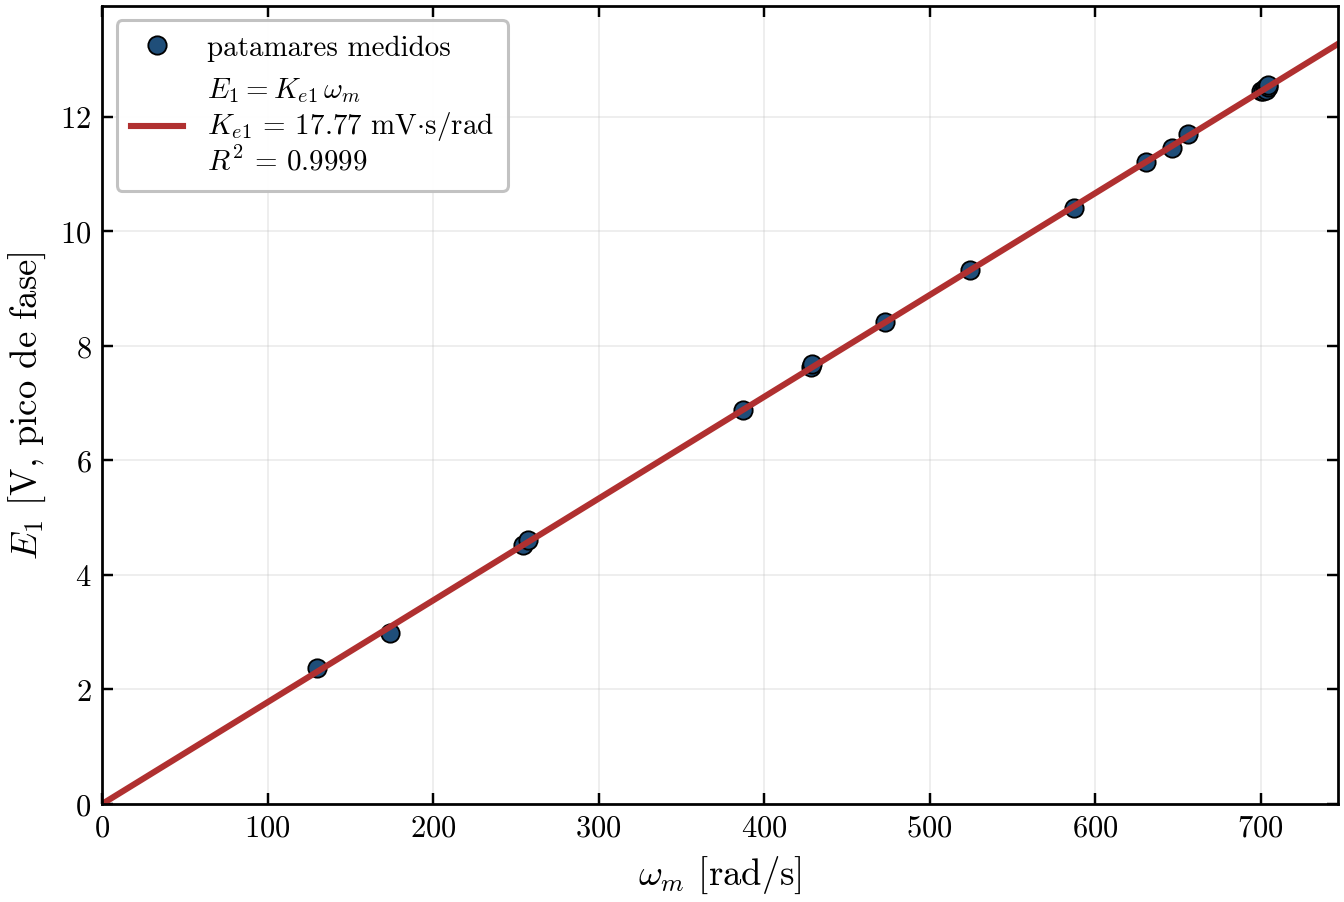
\includegraphics[width=0.9\linewidth]{Textuais/Imgs/Resultados/bancada_ke.png}

    Fonte: Autor (2026)
\end{figure}

\subsection{Projeto das Frequências de Corte do Condicionamento}
\label{sec:resultado_fc}

Os registros de bancada permitiram fixar por medida, e não por estimativa, a
frequência de corte dos filtros que antecedem o conversor analógico-digital.
Sem filtragem, o ruído medido na saída do sensor de corrente é de
\SI{719}{\milli\ampere} rms (\autoref{tab:bancada_parametros}), cerca de quinze vezes o degrau de quantização do
conversor: o ruído sozinho ocupa quatro bits da palavra convertida, de modo
que a filtragem não é um refinamento, e sim condição para que a medida tenha
resolução útil.

A \autoref{fig:bancada_espectros} mostra os espectros de corrente e de tensão
com as faixas de interesse assinaladas: a fundamental elétrica, as raias de
chaveamento do inversor e o patamar de ruído de banda larga que se estende
muito acima delas. É esse patamar, mais do que o conteúdo útil, que orienta
a escolha do corte.

\begin{figure}[H]
    \centering
    \caption{Espectros de corrente e de tensão de fase com as faixas de interesse assinaladas}
    \label{fig:bancada_espectros}
    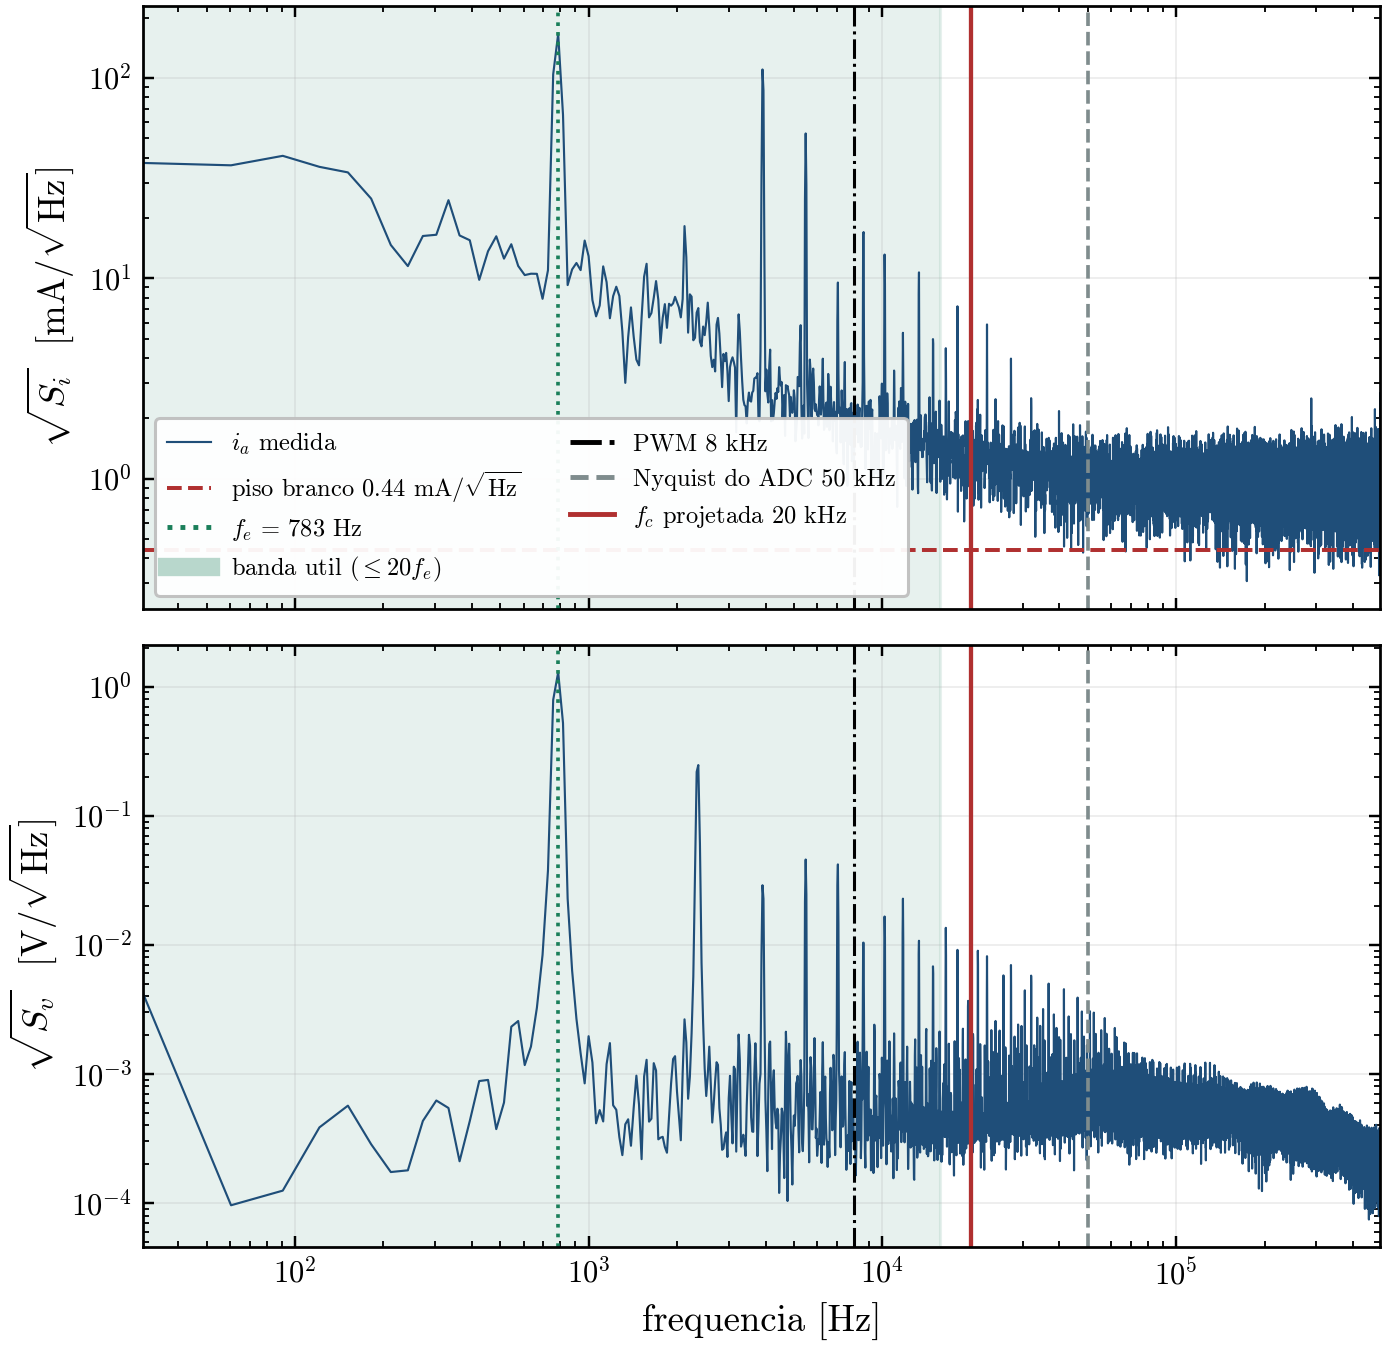
\includegraphics[width=0.9\linewidth]{Textuais/Imgs/Resultados/bancada_espectros.png}

    Fonte: Autor (2026)
\end{figure}

Uma varredura da frequência de corte, com o observador reprocessando os mesmos
registros a cada valor, mostrou que a qualidade da estimação é insensível ao
corte de \SI{3}{\kilo\hertz} para cima.
O motivo é que o próprio observador já é um passa-baixas: o estimador de força
contraeletromotriz tem polo em \SI{1,06}{\kilo\hertz} e a malha de sincronismo
responde a \SI{150}{\hertz}. Tudo o que estiver acima disso é rejeitado pelo
algoritmo, com ou sem filtro analógico. Nessa faixa, portanto, o desempenho
do observador não serve de critério para escolher o corte, que passa a ser
decidido pelo que o observador não tem como desfazer.

São duas as restrições que sobram. A primeira é o rebatimento: componentes
acima de metade da taxa de amostragem retornam à banda de interesse já dentro
da palavra digitalizada, indistinguíveis do sinal, e nenhum processamento
posterior as separa. A segunda é a faixa dinâmica, pelo motivo já exposto: o
ruído que passa pelo filtro consome bits do conversor. As duas restrições
empurram o corte para baixo, enquanto a preservação das raias de chaveamento
o empurra para cima; a \autoref{fig:bancada_restricoes_fc} reúne as três num
mesmo gráfico e delimita a faixa admissível.

\begin{figure}[H]
    \centering
    \caption{Restrições sobre a frequência de corte do condicionamento}
    \label{fig:bancada_restricoes_fc}
    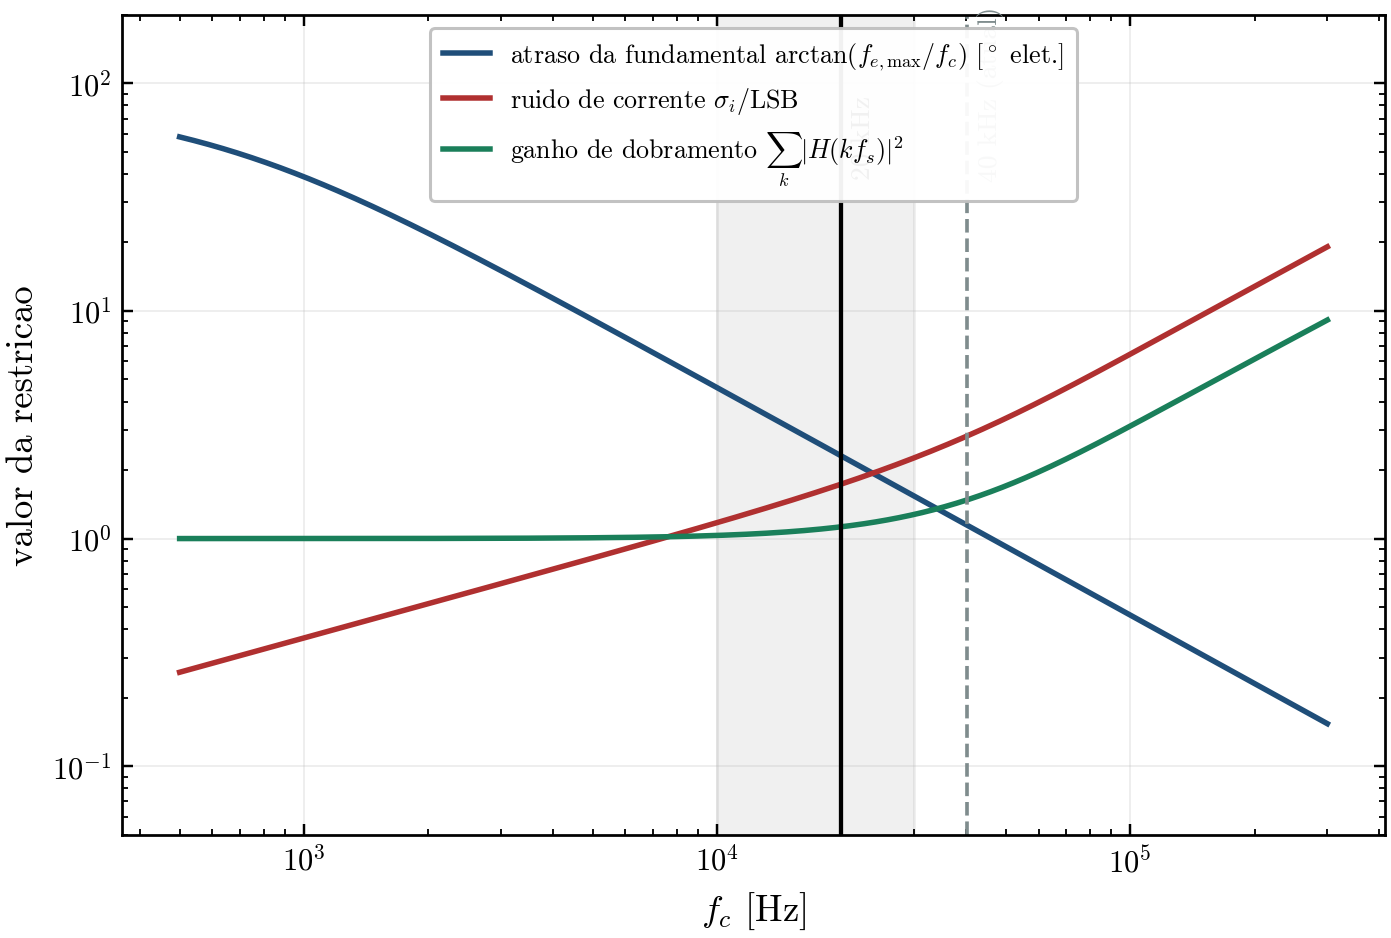
\includegraphics[width=0.9\linewidth]{Textuais/Imgs/Resultados/bancada_restricoes_fc.png}

    Fonte: Autor (2026)
\end{figure}

Adotou-se um filtro de um polo com corte em \SI{20}{\kilo\hertz}, idêntico nos
ramos de tensão e de corrente. A ordem baixa é suficiente porque o observador
complementa a atenuação em alta frequência, e a igualdade entre os dois ramos
é o ponto de atenção do projeto: como o observador extrai a posição da
coerência de fase entre tensão e corrente
(\autoref{sec:condicionamento}), filtros iguais introduzem o mesmo atraso nos
dois caminhos, e o erro de fase entre eles se cancela.

\subsection{Observador Aplicado aos Registros de Bancada}
\label{sec:resultado_smo_bancada}

A última etapa de validação executou o observador sobre os registros da
bancada, alimentando-o com as tensões e correntes medidas no lugar dos sinais
gerados pela simulação. O ensaio é o mesmo dos patamares de rotação em vazio,
de modo que a rotação do tacômetro e o torque do balanço de potência servem de
referência independente para o que o observador estima. A constante de FEM
empregada é a levantada em bancada.

A \autoref{fig:bancada_smo_alfabeta} mostra as correntes, as tensões e a força
contraeletromotriz estimada no referencial estacionário. As componentes
$\alpha$ e $\beta$ da FEM aparecem em quadratura e com amplitude que cresce
com a rotação, comportamento esperado para o sincronismo da malha.

\begin{figure}[H]
    \centering
    \caption{Correntes, tensões e força contraeletromotriz estimada no referencial estacionário}
    \label{fig:bancada_smo_alfabeta}
    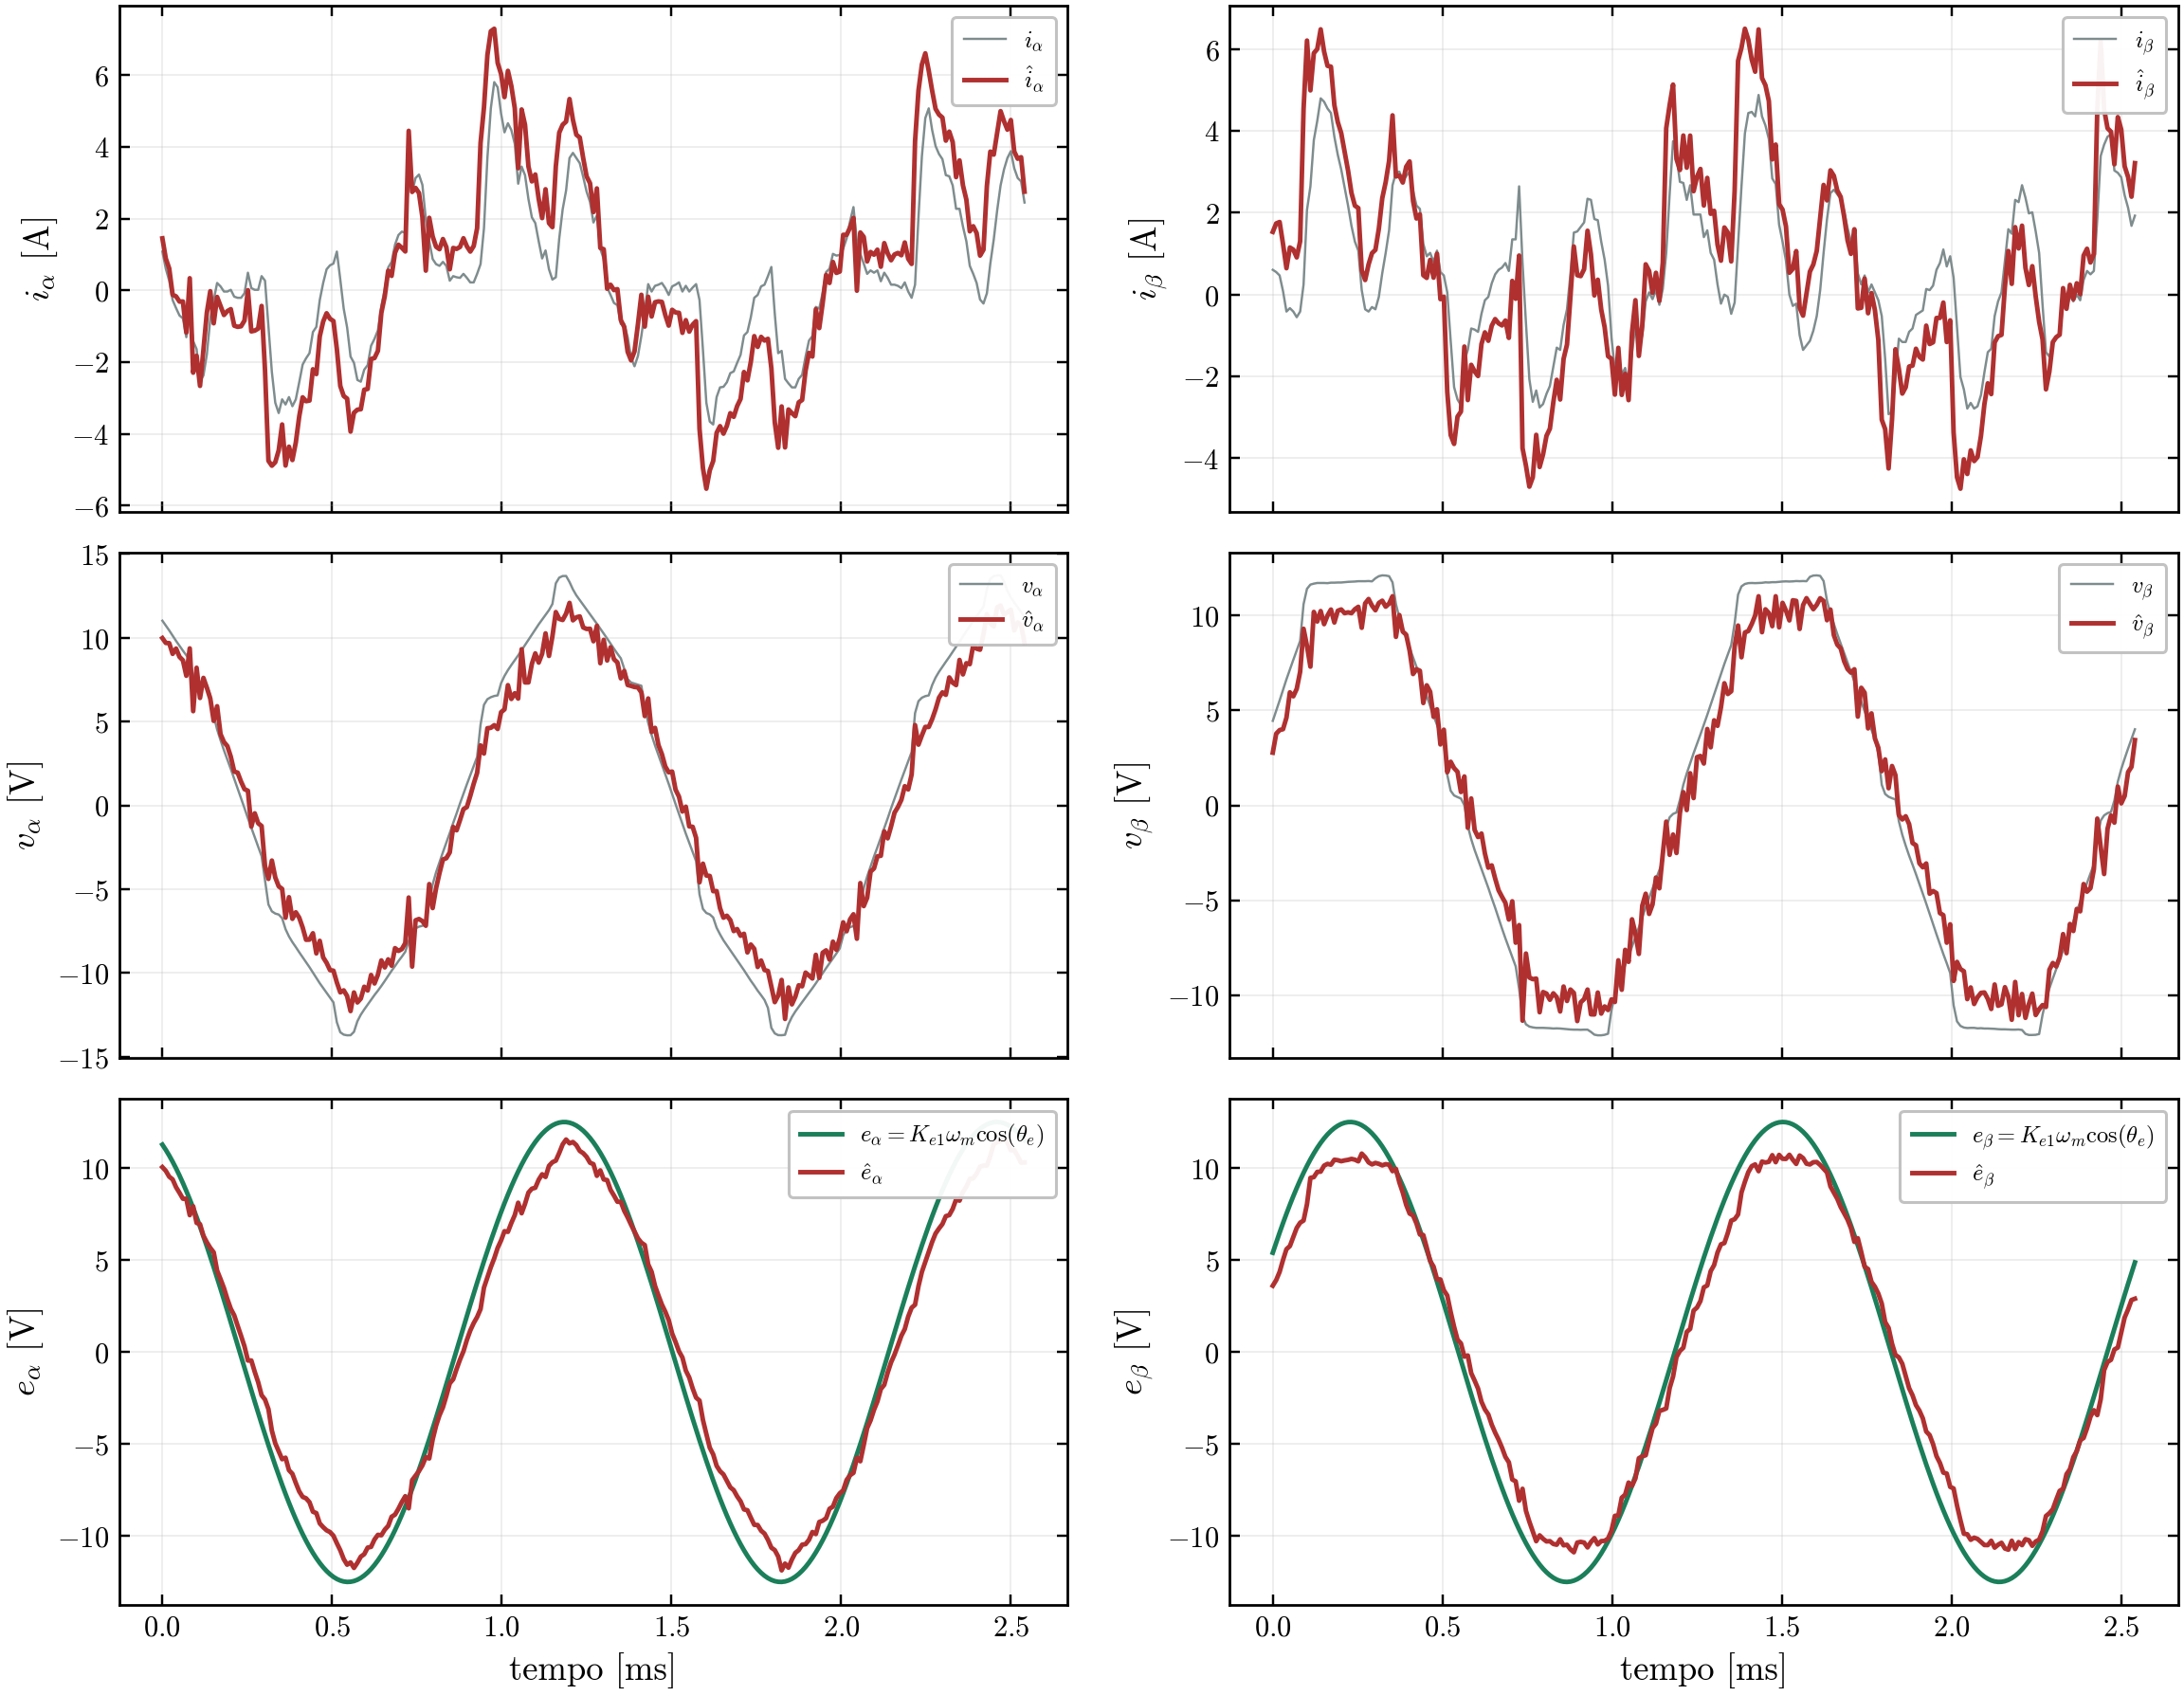
\includegraphics[width=0.9\linewidth]{Textuais/Imgs/Resultados/bancada_smo_alfabeta.png}

    Fonte: Autor (2026)
\end{figure}

A \autoref{fig:bancada_smo_rpm_torque} compara rotação e torque estimados com
os medidos ao longo dos patamares. A velocidade estimada acompanha o tacômetro
com erro médio de \SI{0,092}{\percent}. O torque estimado fica
\SI{-7,2}{\percent} abaixo do medido, resultado obtido projetando a corrente
\emph{medida} sobre o ângulo estimado. Os valores patamar a patamar constam
da \autoref{tab:bancada_smo}, no \autoref{apendice:bancada}.

\begin{figure}[H]
    \centering
    \caption{Rotação e torque, estimados pelo observador e medidos, ao longo dos patamares}
    \label{fig:bancada_smo_rpm_torque}
    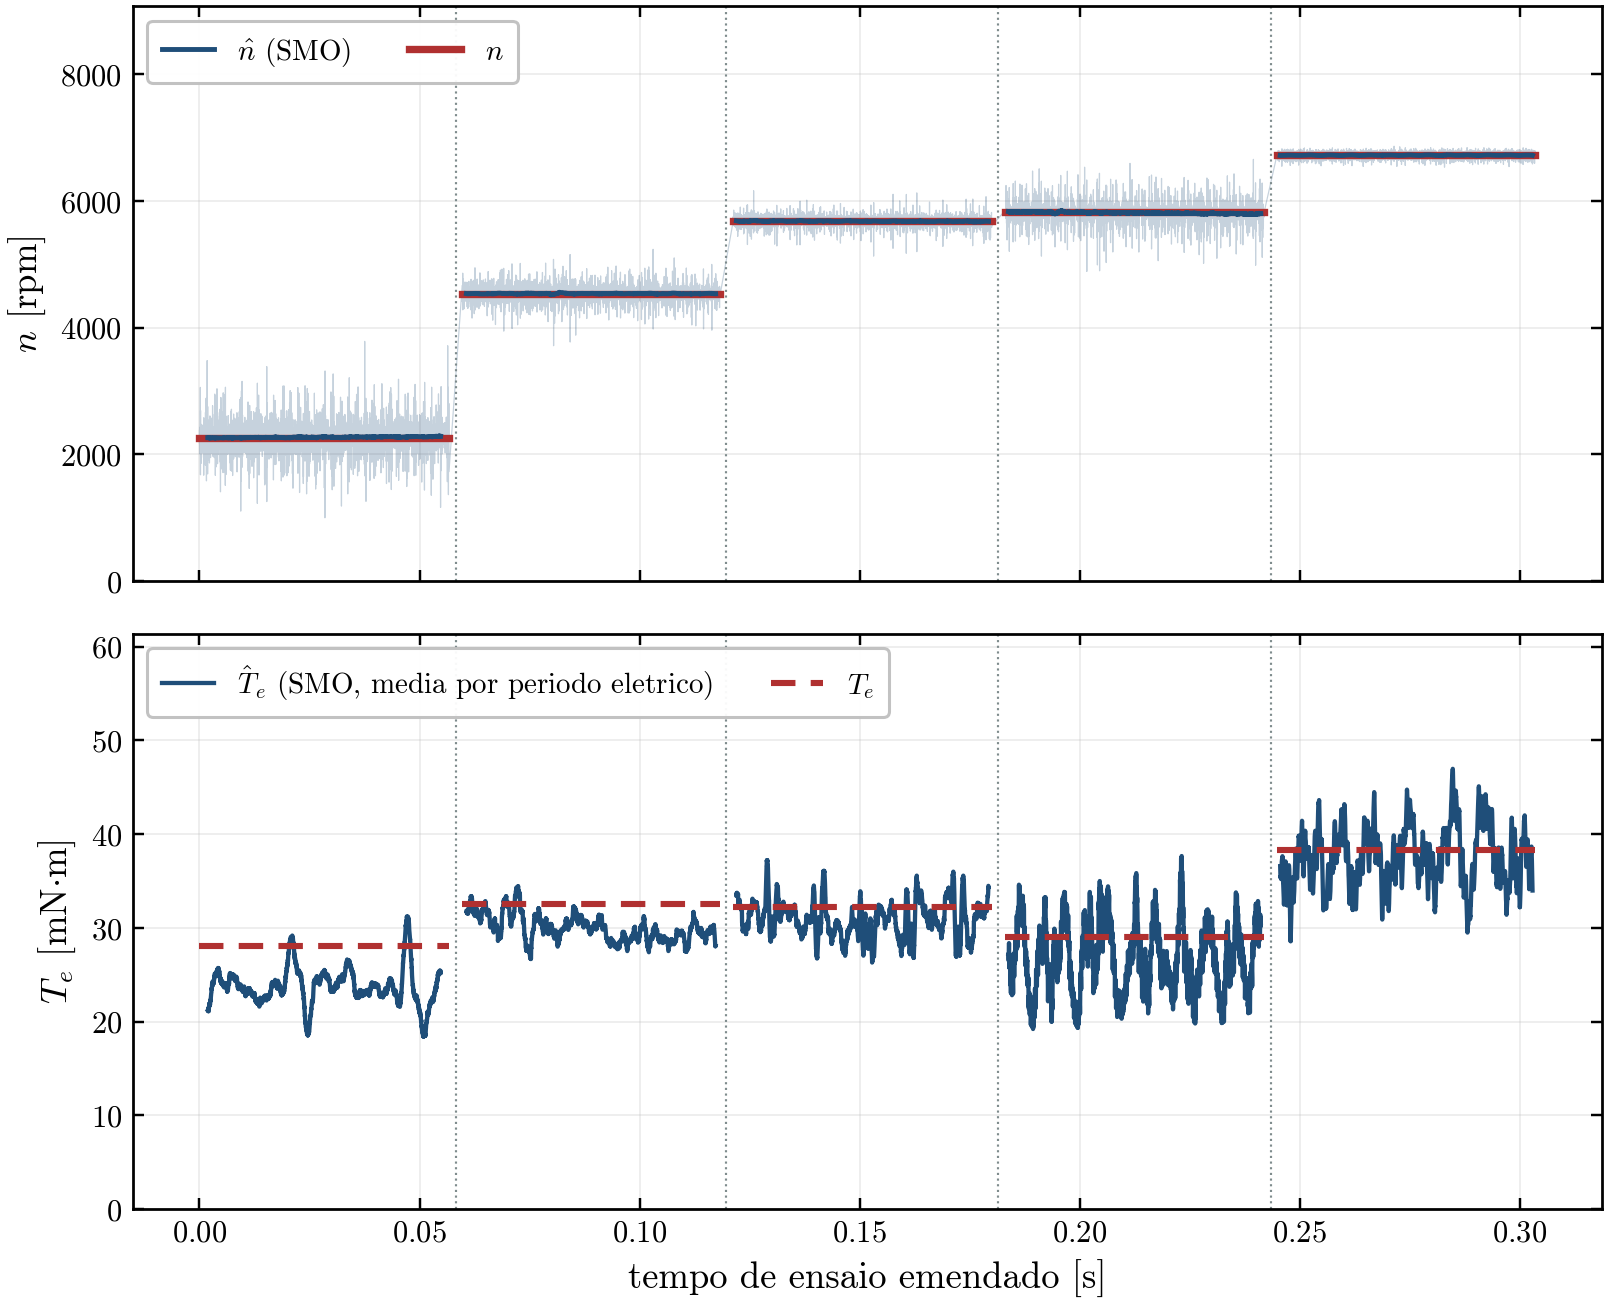
\includegraphics[width=0.9\linewidth]{Textuais/Imgs/Resultados/bancada_smo_rpm_torque.png}

    Fonte: Autor (2026)
\end{figure}

O ângulo elétrico foi conferido contra a integral dos pulsos do tacômetro, que
fornece uma referência de posição independente da estimação. A
\autoref{fig:bancada_smo_angulo_tacometro} traz a comparação em um registro de
\SI{0,5}{\second}: as duas curvas permanecem dentro de \SI{0,3}{\degree} de
diferença média, com comportamento semelhante nos demais patamares
ensaiados.

\begin{figure}[H]
    \centering
    \caption{Ângulo elétrico estimado contra a integral dos pulsos do tacômetro}
    \label{fig:bancada_smo_angulo_tacometro}
    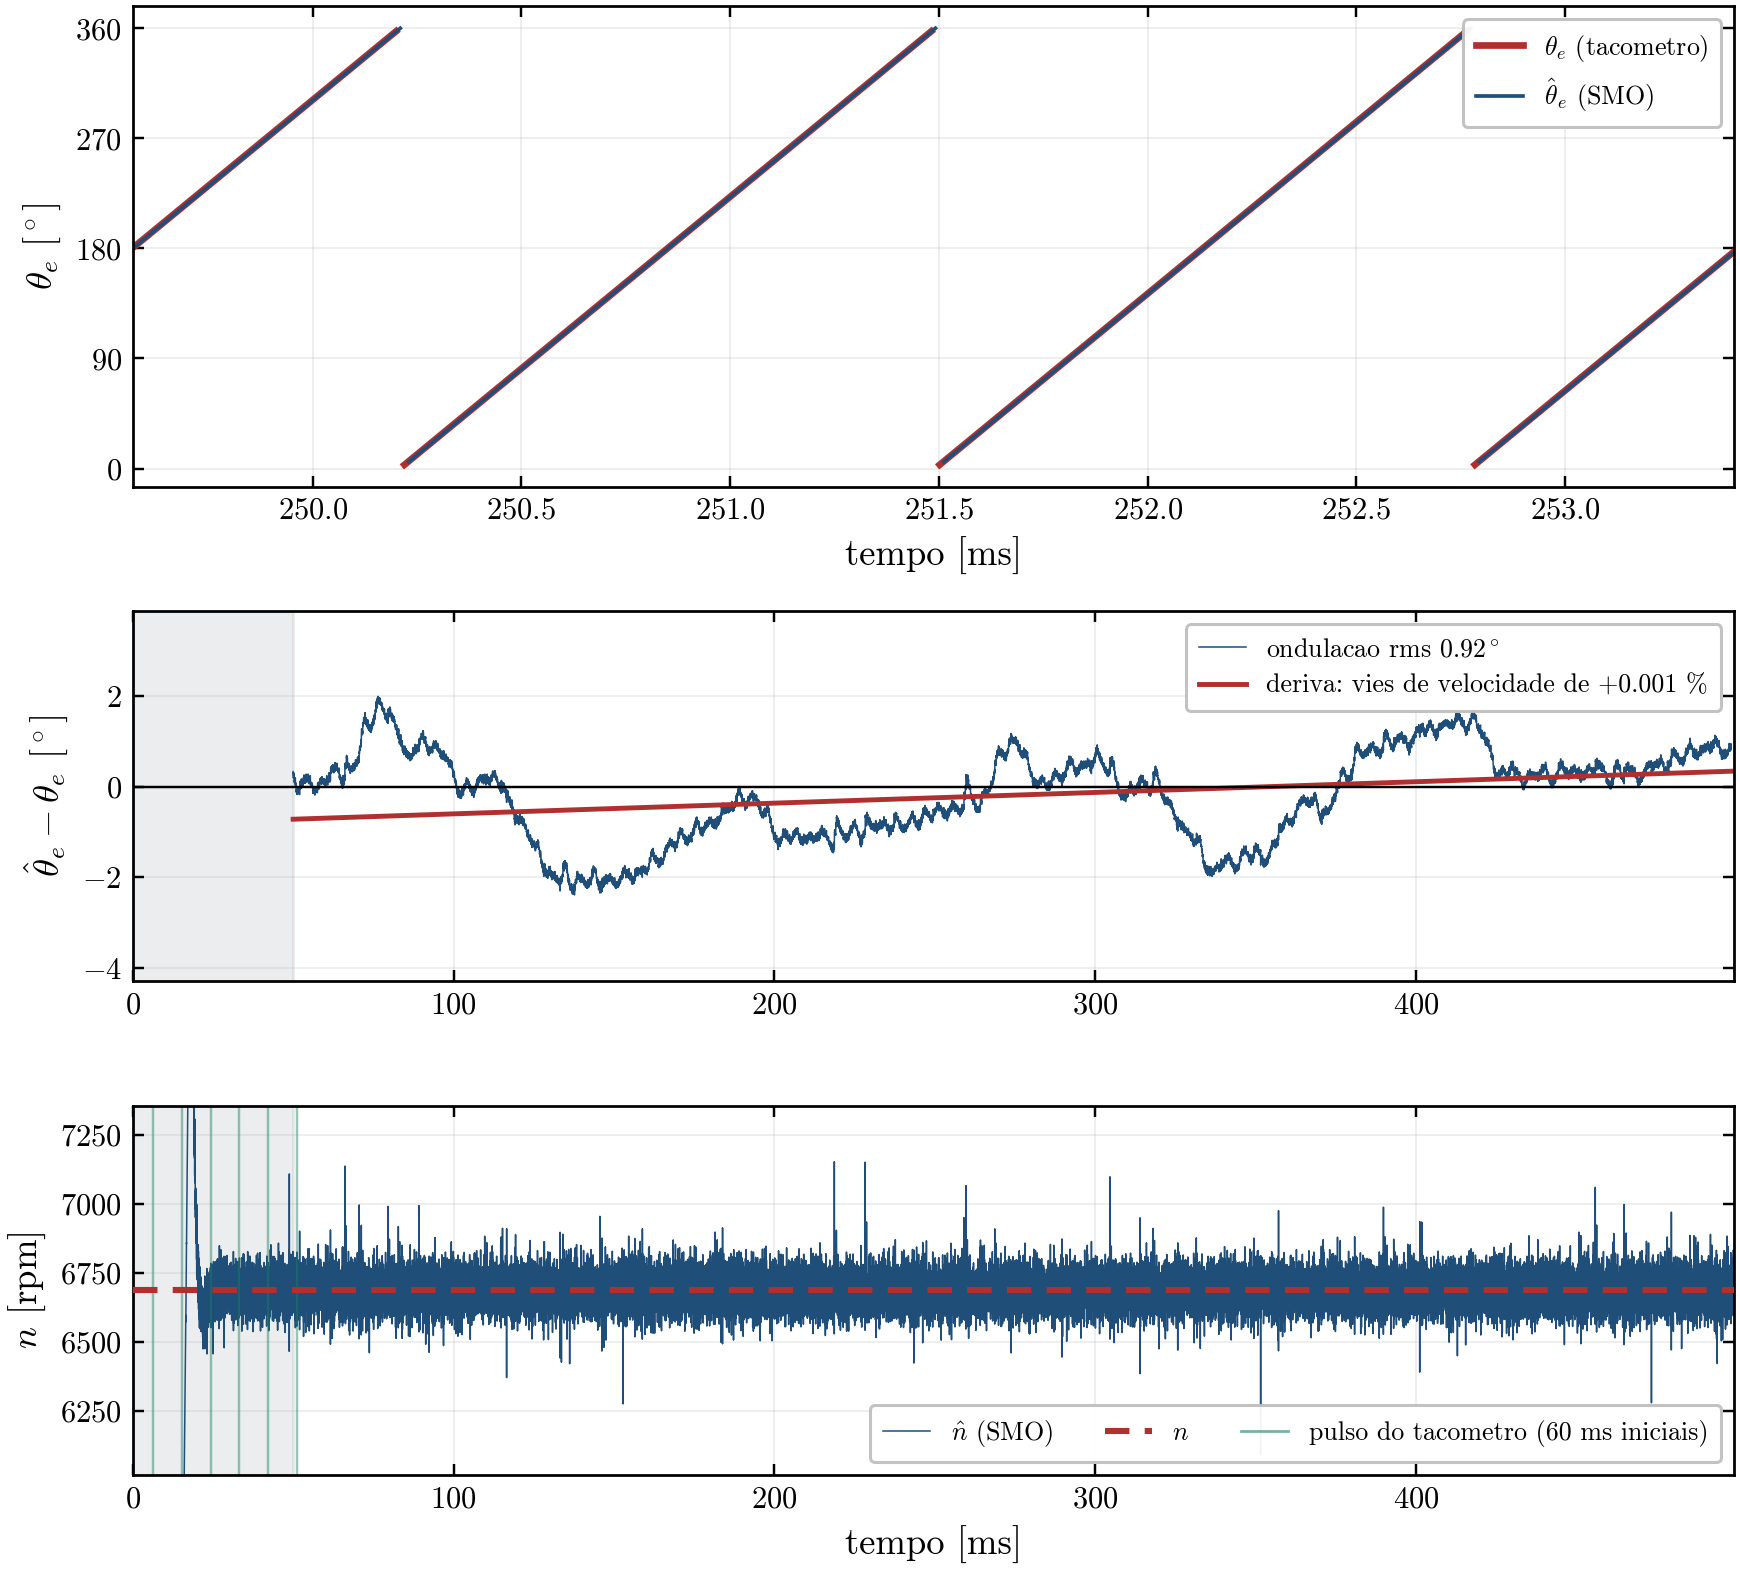
\includegraphics[width=0.9\linewidth]{Textuais/Imgs/Resultados/bancada_smo_angulo_tacometro.png}

    Fonte: Autor (2026)
\end{figure}

Há um limite inferior de operação. A malha de sincronismo responde a
\SI{150}{\hertz}, e abaixo de aproximadamente \num{1930}~RPM o ângulo deixa de
travar na posição do rotor, porque a amplitude da força contraeletromotriz cai
com a rotação e o detector de fase perde referência. A velocidade estimada
continua disponível nessa condição, mas o torque não, já que sua reconstrução
depende da projeção da corrente sobre o ângulo. Na aplicação pretendida ---
caracterização de conjuntos motopropulsores em regime de tração --- a faixa de
interesse está acima desse limite, mas ele precisa ser respeitado na partida e
nas transições de rotação baixa.

\newpage

\subsection{Coeficiente de Torque das Hélices em Bancada}
\label{sec:resultado_coef_aero_bancada}

As hélices APC 15x6E e 17x10E foram ensaiadas na condição estática do
procedimento da \autoref{sec:coef_aero_bancada}, com bateria de seis células.
O acelerador foi levado a três patamares, \SIlist{20;30;40}{\percent}, de
\SI{10}{\second} cada; em cada patamar, descartados os \SI{3}{\second}
iniciais de transitório, a rotação e o torque estimados pelo observador
embarcado foram promediados. O torque da hélice é o estimado menos as perdas a
vazio, $B\,\omega + \tau_c$ (\autoref{sec:resultado_coef_mec}), e $C_Q$ usa
$\rho = \SI{1,225}{\kilo\gram\per\cubic\meter}$. O teórico é a tabela do
fabricante na razão de avanço nula, com $C_Q$ obtido de $C_P$ pela
\autoref{eq:cq_from_cp}. A \autoref{tab:helice_15x6E} e a
\autoref{tab:helice_17x10E} dão os valores e o erro em relação ao teórico; a
\autoref{fig:helice_torque} e a \autoref{fig:helice_cq} mostram as mesmas
grandezas contra a rotação.

\begin{table}[H]
    \centering
    \caption{Torque e coeficiente $C_Q$ da hélice APC 15x6E na condição estática: teórico e bancada}
    \label{tab:helice_15x6E}
    \small
    \setlength{\tabcolsep}{4pt}
    \begin{tabular}{ccccccc}
        \toprule
        & & \multicolumn{2}{c}{\textbf{$Q$ [\si{\newton\meter}]}} & \multicolumn{2}{c}{\textbf{$C_Q$}} & \\
        \cmidrule(lr){3-4}\cmidrule(lr){5-6}
        \textbf{Acelerador} & \textbf{Rotação [RPM]} & \textbf{Teórico} & \textbf{Bancada} & \textbf{Teórico} & \textbf{Bancada} & \textbf{Erro} \\
        \midrule
        \SI{20}{\percent} & \num{1770} & \num{0,0358} & \num{0,0504} $\pm$ \num{0,0034} & \num{0,00418} & \num{0,00589} $\pm$ \num{0,00041} & \SI{+40,7}{\percent} \\
        \SI{30}{\percent} & \num{3050} & \num{0,0953} & \num{0,1191} $\pm$ \num{0,0052} & \num{0,00375} & \num{0,00469} $\pm$ \num{0,00022} & \SI{+25,0}{\percent} \\
        \SI{40}{\percent} & \num{3937} & \num{0,1545} & \num{0,1862} $\pm$ \num{0,0071} & \num{0,00365} & \num{0,00440} $\pm$ \num{0,00019} & \SI{+20,6}{\percent} \\
        \bottomrule
    \end{tabular}

    \vspace{2pt}
    {\small Fonte: Autor (2026); teórico adaptado de \citeonline{apc_performance_data}}
\end{table}

\begin{table}[H]
    \centering
    \caption{Torque e coeficiente $C_Q$ da hélice APC 17x10E na condição estática: teórico e bancada}
    \label{tab:helice_17x10E}
    \small
    \setlength{\tabcolsep}{4pt}
    \begin{tabular}{ccccccc}
        \toprule
        & & \multicolumn{2}{c}{\textbf{$Q$ [\si{\newton\meter}]}} & \multicolumn{2}{c}{\textbf{$C_Q$}} & \\
        \cmidrule(lr){3-4}\cmidrule(lr){5-6}
        \textbf{Acelerador} & \textbf{Rotação [RPM]} & \textbf{Teórico} & \textbf{Bancada} & \textbf{Teórico} & \textbf{Bancada} & \textbf{Erro} \\
        \midrule
        \SI{20}{\percent} & \num{1335} & \num{0,0573} & \num{0,0688} $\pm$ \num{0,0037} & \num{0,00630} & \num{0,00756} $\pm$ \num{0,00043} & \SI{+20,0}{\percent} \\
        \SI{30}{\percent} & \num{2308} & \num{0,1512} & \num{0,1758} $\pm$ \num{0,0066} & \num{0,00556} & \num{0,00646} $\pm$ \num{0,00027} & \SI{+16,3}{\percent} \\
        \SI{40}{\percent} & \num{3010} & \num{0,2431} & \num{0,2888} $\pm$ \num{0,0099} & \num{0,00525} & \num{0,00624} $\pm$ \num{0,00025} & \SI{+18,8}{\percent} \\
        \bottomrule
    \end{tabular}

    \vspace{2pt}
    {\small Fonte: Autor (2026); teórico adaptado de \citeonline{apc_performance_data}}
\end{table}

% Pontos medidos: Textuais/Imgs/Resultados/helice/medido_<hélice>.dat (torque do
% observador já corrigido para o divisor de 9,1 kOhm). Perdas: B = 32,4e-6 N.m.s/rad,
% tau_c = 15,5e-3 N.m. D^5: 15" = 8,028e-3 m^5; 17" = 1,5011e-2 m^5.
\pgfplotsset{
    helice/.style={width=\linewidth, height=5.5cm, grid=both,
        grid style={dotted,gray!40}, xmin=1000, xtick distance=1000, legend pos=north west,
        legend style={font=\scriptsize}, tick label style={font=\scriptsize},
        label style={font=\small}, xlabel={Rotação [RPM]},
        scaled x ticks=false, xticklabel style={/pgf/number format/1000 sep={}}},
    tabhelice/.style={table/comment chars={\#}},
    apcfaixa/.style={restrict x to domain=1000:4000},
    barras/.style={error bars/.cd, x dir=both, x explicit, y dir=both, y explicit,
        error bar style={line width=0.8pt}, error mark options={rotate=90, mark size=3pt, line width=0.8pt}},
}

\begin{figure}[H]
    \centering
    \caption{Torque aerodinâmico das hélices na condição estática: teórico e bancada}
    \label{fig:helice_torque}
    \begin{subfigure}[t]{0.49\textwidth}
        \centering
        \begin{tikzpicture}
        \begin{axis}[helice, xmax=4000, ylabel={$Q$ [\si{\newton\meter}]}, ymin=0]
            \addplot[thick, blue!65!black, apcfaixa] table[x=rpm, y=torque_Nm] {Textuais/Imgs/Resultados/helice/apc_15x6E_estatico.dat};
            \addlegendentry{APC (teórico)}
            \addplot[only marks, mark=*, blue!65!black, barras] table[tabhelice, x=rpm,
                y expr={\thisrow{Te_Nm} - (32.4e-6*\thisrow{rpm}*0.1047198 + 15.5e-3)},
                x error=rpm_err, y error expr={sqrt(\thisrow{Te_err}^2 + (0.03*\thisrow{Te_Nm})^2 + (4.4e-6*\thisrow{rpm}*0.1047198)^2 + (2.4e-3)^2)}]
                {Textuais/Imgs/Resultados/helice/medido_15x6E.dat};
            \addlegendentry{bancada}
            \addplot[thick, dashed, black!70, domain=1000:4000, samples=60] {2.5924e-07*x^1.627};
            \addlegendentry{ajuste $Q \propto n^{1,63}$}
        \end{axis}
        \end{tikzpicture}
        \caption{APC 15x6E}
    \end{subfigure}
    \hfill
    \begin{subfigure}[t]{0.49\textwidth}
        \centering
        \begin{tikzpicture}
        \begin{axis}[helice, xmax=4000, ylabel={$Q$ [\si{\newton\meter}]}, ymin=0]
            \addplot[thick, red!65!black, apcfaixa] table[x=rpm, y=torque_Nm] {Textuais/Imgs/Resultados/helice/apc_17x10E_estatico.dat};
            \addlegendentry{APC (teórico)}
            \addplot[only marks, mark=square*, red!65!black, barras] table[tabhelice, x=rpm,
                y expr={\thisrow{Te_Nm} - (32.4e-6*\thisrow{rpm}*0.1047198 + 15.5e-3)},
                x error=rpm_err, y error expr={sqrt(\thisrow{Te_err}^2 + (0.03*\thisrow{Te_Nm})^2 + (4.4e-6*\thisrow{rpm}*0.1047198)^2 + (2.4e-3)^2)}]
                {Textuais/Imgs/Resultados/helice/medido_17x10E.dat};
            \addlegendentry{bancada}
            \addplot[thick, dashed, black!70, domain=1000:4000, samples=60] {2.2085e-07*x^1.757};
            \addlegendentry{ajuste $Q \propto n^{1,76}$}
        \end{axis}
        \end{tikzpicture}
        \caption{APC 17x10E}
    \end{subfigure}

    Fonte: Autor (2026)
\end{figure}

\begin{figure}[H]
    \centering
    \caption{Coeficiente de torque $C_Q$ das hélices na condição estática: teórico e bancada}
    \label{fig:helice_cq}
    \begin{subfigure}[t]{0.49\textwidth}
        \centering
        \begin{tikzpicture}
        \begin{axis}[helice, xmax=4000, ylabel={$C_Q$}, ymin=0.003, ymax=0.0068, legend pos=north east,
                     yticklabel style={/pgf/number format/fixed, /pgf/number format/precision=4}]
            \addplot[thick, blue!65!black, apcfaixa] table[x=rpm, y=CQ] {Textuais/Imgs/Resultados/helice/apc_15x6E_estatico.dat};
            \addlegendentry{APC (teórico)}
            \addplot[only marks, mark=*, blue!65!black, barras] table[tabhelice, x=rpm,
                y expr={(\thisrow{Te_Nm} - (32.4e-6*\thisrow{rpm}*0.1047198 + 15.5e-3)) / (\thisrow{rho}*(\thisrow{rpm}/60)^2*8.0283e-3)},
                x error=rpm_err,
                y error expr={sqrt(\thisrow{Te_err}^2 + (0.03*\thisrow{Te_Nm})^2 + (4.4e-6*\thisrow{rpm}*0.1047198)^2 + (2.4e-3)^2
                        + (0.02*(\thisrow{Te_Nm} - (32.4e-6*\thisrow{rpm}*0.1047198 + 15.5e-3)))^2) / (\thisrow{rho}*(\thisrow{rpm}/60)^2*8.0283e-3)}]
                {Textuais/Imgs/Resultados/helice/medido_15x6E.dat};
            \addlegendentry{bancada}
            \addplot[thick, dashed, black!70, domain=1000:4000, samples=60] {2.5924e-07*x^1.627 / (1.225*(x/60)^2*8.0283e-3)};
            \addlegendentry{ajuste}
        \end{axis}
        \end{tikzpicture}
        \caption{APC 15x6E}
    \end{subfigure}
    \hfill
    \begin{subfigure}[t]{0.49\textwidth}
        \centering
        \begin{tikzpicture}
        \begin{axis}[helice, xmax=4000, ylabel={$C_Q$}, ymin=0.004, ymax=0.0085, legend pos=north east,
                     yticklabel style={/pgf/number format/fixed, /pgf/number format/precision=4}]
            \addplot[thick, red!65!black, apcfaixa] table[x=rpm, y=CQ] {Textuais/Imgs/Resultados/helice/apc_17x10E_estatico.dat};
            \addlegendentry{APC (teórico)}
            \addplot[only marks, mark=square*, red!65!black, barras] table[tabhelice, x=rpm,
                y expr={(\thisrow{Te_Nm} - (32.4e-6*\thisrow{rpm}*0.1047198 + 15.5e-3)) / (\thisrow{rho}*(\thisrow{rpm}/60)^2*1.50111e-2)},
                x error=rpm_err,
                y error expr={sqrt(\thisrow{Te_err}^2 + (0.03*\thisrow{Te_Nm})^2 + (4.4e-6*\thisrow{rpm}*0.1047198)^2 + (2.4e-3)^2
                        + (0.02*(\thisrow{Te_Nm} - (32.4e-6*\thisrow{rpm}*0.1047198 + 15.5e-3)))^2) / (\thisrow{rho}*(\thisrow{rpm}/60)^2*1.50111e-2)}]
                {Textuais/Imgs/Resultados/helice/medido_17x10E.dat};
            \addlegendentry{bancada}
            \addplot[thick, dashed, black!70, domain=1000:4000, samples=60] {2.2085e-07*x^1.757 / (1.225*(x/60)^2*1.50111e-2)};
            \addlegendentry{ajuste}
        \end{axis}
        \end{tikzpicture}
        \caption{APC 17x10E}
    \end{subfigure}

    Fonte: Autor (2026)
\end{figure}

O torque e o $C_Q$ de bancada seguem a forma das curvas teóricas, com o
torque crescendo com a rotação e o $C_Q$ diminuindo levemente, e ficam acima
delas: de \SIrange{16}{20}{\percent} na 17x10E e de \SIrange{21}{41}{\percent}
na 15x6E. A curva tracejada é o ajuste $Q = a\,n^{b}$ aos pontos de cada
hélice, com expoente $b = \num{1,63}$ na 15x6E e $b = \num{1,76}$ na 17x10E,
contra cerca de \num{1,87} no teórico entre \SIlist{1000;4000}{RPM}. Essas
diferenças são discutidas na \autoref{sec:discussao_helices}.

As barras de erro somam o desvio-padrão no patamar, a incerteza de $B$ e
$\tau_c$, \SI{3}{\percent} no ganho dos sensores de corrente e, no $C_Q$,
\SI{2}{\percent} na densidade do ar. A \autoref{fig:helice_gui} mostra os dois
registros como aparecem na interface, a partir do degrau de \SI{20}{\percent},
o primeiro que põe o motor em rotação. As tensões e correntes são amostras
isoladas a \SI{10}{\hertz}, cada uma num instante qualquer do chaveamento, e
não a forma de onda.

\begin{figure}[H]
    \centering
    \caption{Registros dos ensaios das hélices exibidos na interface de usuário}
    \label{fig:helice_gui}
    \begin{subfigure}[t]{\textwidth}
        \centering
        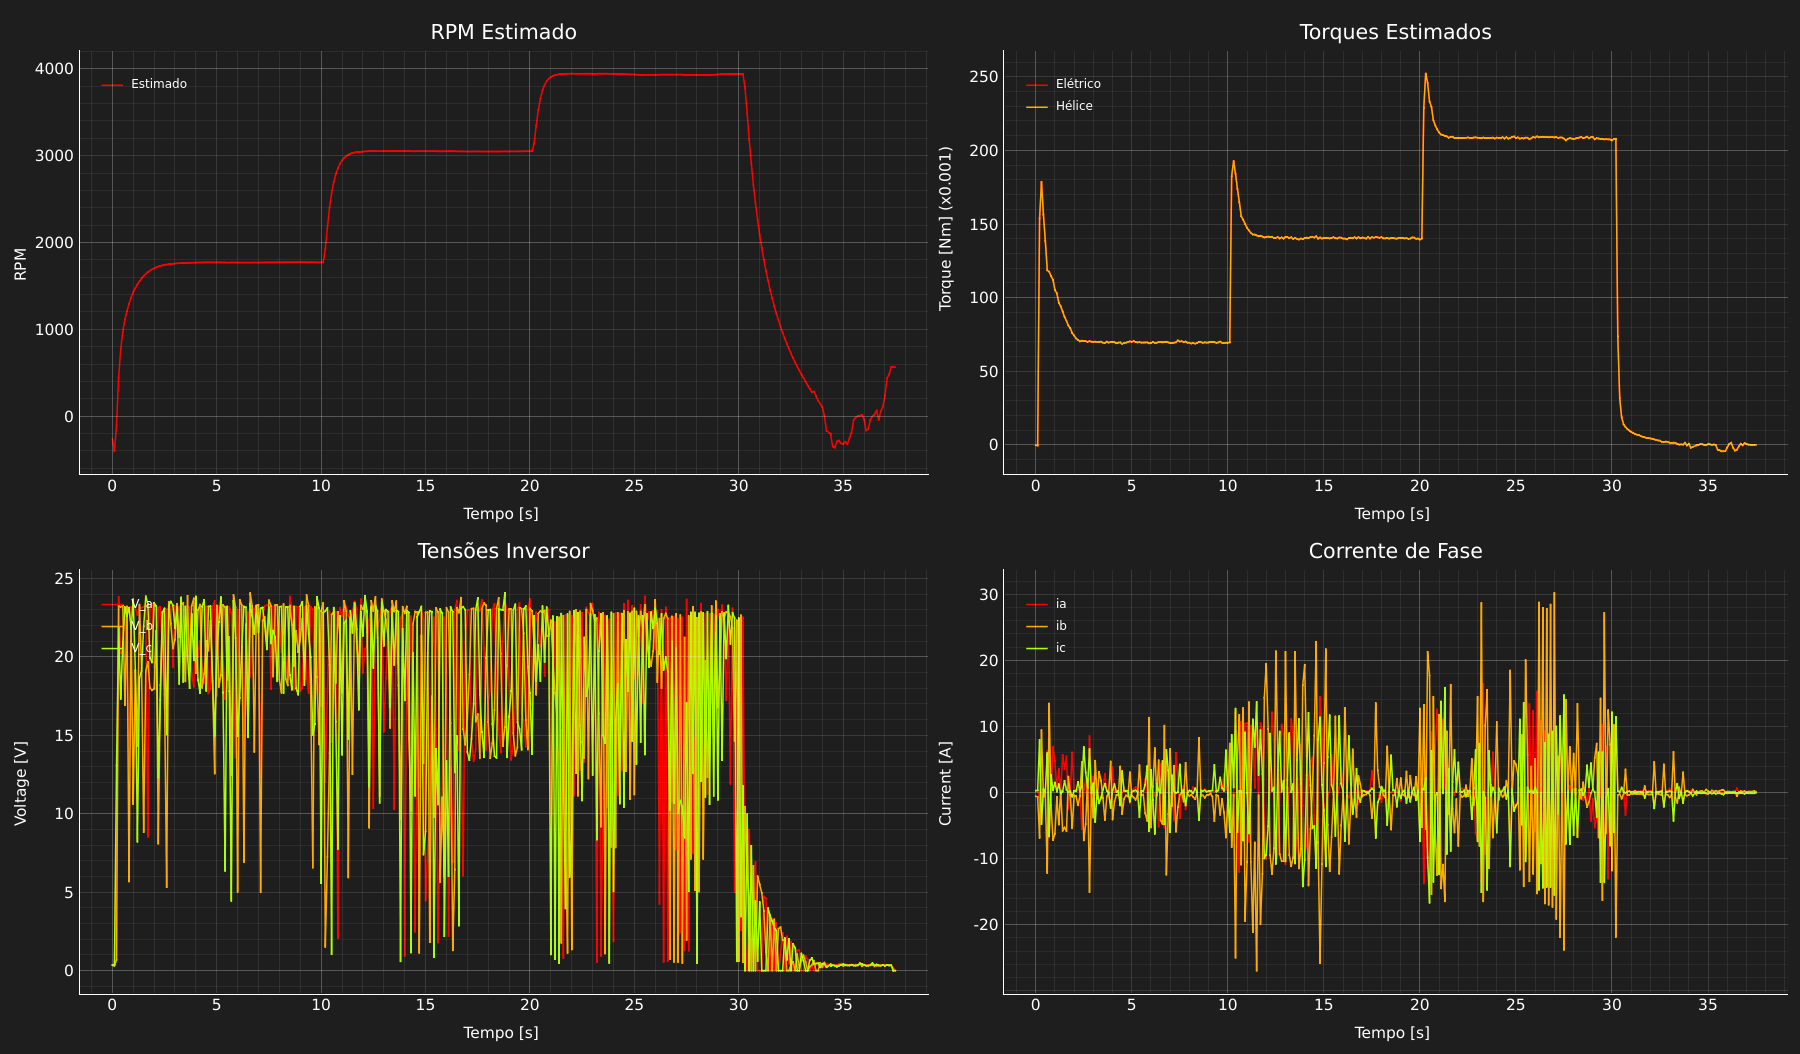
\includegraphics[width=0.95\linewidth]{Textuais/Imgs/Resultados/helice/gui_ensaio_15x6E.png}
        \caption{APC 15x6E}
    \end{subfigure}

    \vspace{0.3cm}
    \begin{subfigure}[t]{\textwidth}
        \centering
        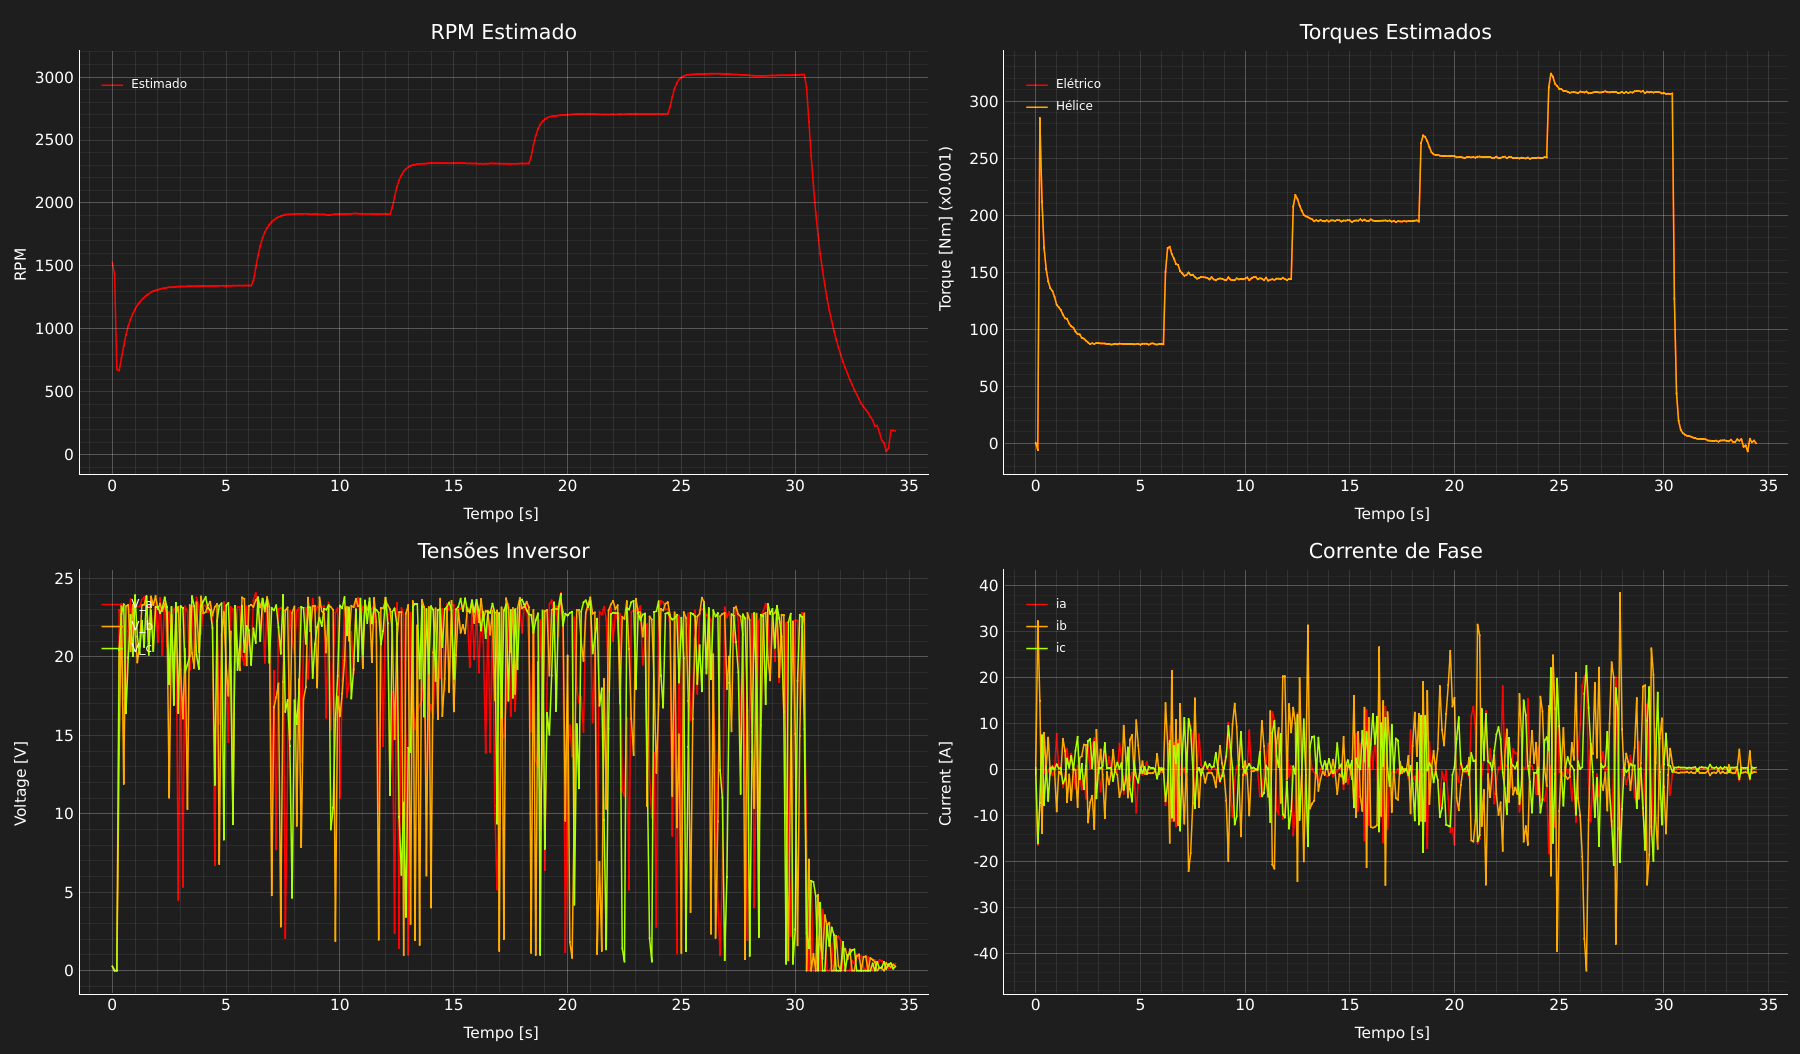
\includegraphics[width=0.95\linewidth]{Textuais/Imgs/Resultados/helice/gui_ensaio_17x10E.png}
        \caption{APC 17x10E}
    \end{subfigure}

    Fonte: Autor (2026)
\end{figure}
